%Copyright 2019 Christopher M. Jermaine (cmj4@rice.edu) and Risa B. Myers (rbm2@rice.edu)
%
%Licensed under the Apache License, Version 2.0 (the "License");
%you may not use this file except in compliance with the License.
%You may obtain a copy of the License at
%
%    https://www.apache.org/licenses/LICENSE-2.0
%
%Unless required by applicable law or agreed to in writing, software
%distributed under the License is distributed on an "AS IS" BASIS,
%WITHOUT WARRANTIES OR CONDITIONS OF ANY KIND, either express or implied.
%See the License for the specific language governing permissions and
%limitations under the License.

\documentclass[aspectratio=169]{beamer}

%===============================================================%
\mode<presentation> 
{
\usetheme[noshadow, minimal,numbers,riceb,nonav]{Rice}
\usefonttheme[onlymath]{serif}
\setbeamercovered{transparent}
}
\useinnertheme{rectangles}

\usepackage[english]{babel}
\usepackage{colortbl}

\usepackage{mathptmx}
\usepackage{helvet}
\usepackage{courier}
\usepackage[T1]{fontenc}
\usepackage{trajan}
\setbeamerfont{block body}{size=\tiny}
\definecolor{midgreen}{rgb}{0.0, 0.5, 0.0}

\usepackage{textcomp}
\usepackage{ulem}
\usepackage{multirow}

\usepackage{listings}
\newenvironment{noindentitemize}
{ \begin{itemize}
 \setlength{\itemsep}{1.5ex}
  \setlength{\parsep}{0pt}   
  \setlength{\parskip}{0pt}
 \addtolength{\leftskip}{-2em}
 }
{ \end{itemize} }

\newenvironment{noindentitemize2}
{ \begin{itemize}
  \setlength{\itemsep}{0ex}
  \setlength{\parskip}{0pt}
  \setlength{\parsep}{0pt}   
  \addtolength{\leftskip}{-2em}  }
{ \end{itemize} }



\lstnewenvironment{SQL}
  {\lstset{
        aboveskip=5pt,
        belowskip=5pt,
        escapechar=!,
        mathescape=true,
        upquote=true,
        language=SQL,
        basicstyle=\linespread{0.94}\ttfamily\footnotesize,
        morekeywords={PRINT, CURSOR, OPEN, FETCH, CLOSE, DECLARE, BEGIN, END, PROCEDURE, FOR, EACH, WITH, PARTITION, TEST, WHETHER, PROBABILITY, OUT,LOOP,IF,CONTINUE, HANDLER,CALL,FUNCTION, RETURNS, RETURN, BEFORE, ROW, OUT, 
        DELIMITER,CONCAT,FOUND,LEAVE, HANDLER, DOUBLE, TEMPORARY, REFERENCES },
        deletekeywords={VALUE, PRIOR},
        showstringspaces=true}
        \vspace{0pt}%
        \noindent\minipage{0.47\textwidth}}
  {\endminipage\vspace{0pt}}
  
\lstnewenvironment{SQLtiny}
  {\lstset{
        aboveskip=5pt,
        belowskip=5pt,
        escapechar=!,
        mathescape=true,
        upquote=true,
        language=SQL,
        basicstyle=\linespread{0.94}\ttfamily\tiny,
        morekeywords={PRINT, CURSOR, OPEN, FETCH, CLOSE, DECLARE, BEGIN, END, PROCEDURE, FOR, EACH, WITH, PARTITION, TEST, WHETHER, PROBABILITY, OUT,LOOP,IF,CONTINUE, HANDLER,CALL, FUNCTION, RETURNS, LANGUAGE,BODY,RETURN,
        EXIT, TEXT, REFCURSOR, QUOTE_LITERAL, DELIMITER,CONCAT,FOUND,LEAVE },
        deletekeywords={VALUE, PRIOR},
        showstringspaces=true}
        \vspace{0pt}%
        \noindent\minipage{0.47\textwidth}}
  {\endminipage\vspace{0pt}}

\newcommand{\FACULTY}{\textrm{FACULTY}} 
\newcommand{\STUDENT}{\textrm{STUDENT}} 
\newcommand{\ENROLL}{\textrm{ENROLL}} 
\newcommand{\COURSE}{\textrm{COURSE}} 
\newcommand{\TEACHES}{\textrm{TEACHES}} 
\newcommand{\LIKES}{\textrm{LIKES}} 
\newcommand{\FREQUENTS}{\textrm{FREQUENTS}} 
\newcommand{\SERVES}{\textrm{SERVES}} 
\newcommand{\CAFE}{\textrm{CAFE}} 
\newcommand{\COFFEE}{\textrm{COFFEE}} 
\newcommand{\DRINKER}{\textrm{DRINKER}} 
\newcommand{\CB}{\textrm{\textquotesingle{Cold Brew}\textquotesingle}} 
\newcommand{\CBGOOD}{\textrm{CBGOOD}} 
\newcommand{\ALLPEEPS}{\textrm{ALLPEEPS}} 
\newcommand{\ALLCOMBOS}{\textrm{ALLCOMBOS}} 
\newcommand{\GOODCOFFEE}{\textrm{GOODCOFFEE}} 



%===============================================================%

\title[]
{Tools \& Models for Data Science}

\subtitle
{Relational Algebra}

\author[]{Chris Jermaine \& Risa Myers}
\institute
{
  Rice University
}

\date[]{}


\begin{document}

\begin{frame}
 \titlepage
\end{frame}

%***********************************************************

\begin{frame}{Relational Calculus vs. Algebra}

\begin{itemize}
\item In Relational Calculus
	\begin{itemize}
	\item You say what you want
	\item And not how to compute it
	\end{itemize}
\item But obviously...
	\begin{itemize}
	\item This needs to be compiled into an actual computational plan
	\item And in relational DBs, the plan is expressed in relational algebra
	\end{itemize}
\item RA is the ``abstract machine'' of relational databases
\end{itemize}
\end{frame}

%***********************************************************
\begin{frame}{What Is An Algebra?}

\begin{itemize}
\item Many Definitions!
	\begin{itemize}
	\item Simplest: it is a set (domain) with a number of operations
	\item The domain is closed under those operations
	\end{itemize}
\item In RA...
	\begin{itemize}
	\item The domain is the set of all valid relations
	\item The set of operations includes $\pi, \sigma, \times, \bowtie, \cup, \cap, -$
	\end{itemize}
\item Now let's go through the operations!
\end{itemize}
\end{frame}

%***********************************************************
\begin{frame}{Projection}

\begin{itemize}
\item Projection removes attributes
\item $\pi_A (R)$...
	\begin{itemize}
	\item $A$ is a set of attributes of relation $R$
	\item This simply removes all attributes not in $A$ from $R$
	\item Note: cardinality of output can differ from $R$
	\item Output is a relation
	\end{itemize}
\end{itemize}
\end{frame}
%***********************************************************
\begin{frame}{Projection Example}

COURSE(\underline{CRN}, NAME, DOW, STARTTIME, ENDTIME)

\begin{enumerate}
\item Return course names

$\pi_{name}(\textrm{COURSE})$

\{(\textquotesingle{Comp430}\textquotesingle), (\textquotesingle{Comp}140\textquotesingle), ...\}
\item Return course name and days of the week when courses meet

$\pi_{name, dow}(\textrm{COURSE})$

\{(\textquotesingle{Comp430}\textquotesingle, \textquotesingle{MWF}\textquotesingle), (\textquotesingle{Comp}140\textquotesingle, \textquotesingle{TR}\textquotesingle), ...)\}
\end{enumerate}
\end{frame}


%***********************************************************
\begin{frame}{Projection Visualization}

COURSE\\
\begin{tabular}{|p{1.5cm}|l|l|p{2cm}|p{2cm}|}  \hline
\textrm{CRN} & \textrm{NAME} & \textrm{DOW}& \textrm{STARTTIME}& \textrm{ENDTIME}\\ \hline
 12809 & COMP 430 & MWF & 14:00:00 & 14:50:00 \\ \hline
 12810 & COMP 533 & MWF & 14:00:00 & 14:50:00 \\ \hline
 10396 & COMP 140 & TR & 10:50:00 & 12:05:00 \\ \hline
 13970 & COMP 436 & WF & 14:30:00 & 15:45:00 \\ \hline
\end{tabular}

\vspace{1em}
$\pi_{name, dow}(\textrm{COURSE})$
\vspace{1em}

\begin{tabular}{|p{1.5cm}|l|l|p{2cm}|p{2cm}|}  \hline
\cellcolor{black} & \textrm{NAME} & \textrm{DOW}& \cellcolor{black}&\cellcolor{black}\\ \hline
\cellcolor{black}  & COMP 430 & MWF & \cellcolor{black} & \cellcolor{black} \\ \hline
 \cellcolor{black} & COMP 533 & MWF & \cellcolor{black} &\cellcolor{black} \\ \hline
 \cellcolor{black} & COMP 140 & TR & \cellcolor{black} & \cellcolor{black} \\ \hline
 \cellcolor{black} & COMP 436 & WF & \cellcolor{black} & \cellcolor{black} \\ \hline
\end{tabular}

%\begin{columns}[t]
%\begin{column}{0.5\textwidth}
%FREQUENTS\\
%\begin{tabular}{|l|l|}  \hline
%\textrm{DRINKER} & \textrm{CAFE} \\ \hline
% Risa & JL \\ \hline
% Risa & BH \\ \hline
%Chris & BH \\ \hline
%Chris & DT \\ \hline % double trouble
%\end{tabular}
%\end{column}
%\begin{column}{0.5\textwidth}
%$\pi_{\textrm{DRINKER}}(\textrm{FREQUENTS})$\\
%\begin{tabular}{|l|l|}  \hline
%\textrm{DRINKER} \\ \hline
% Risa \\ \hline
%Chris  \\ \hline % double trouble
%\end{tabular}
%\end{column}
%\end{columns}

\end{frame}

%***********************************************************
\begin{frame}{Selection}

\begin{itemize}
\item Selection removes tuples
\item $\sigma_B (R)$...
	\begin{itemize}
	\item $B$ is a boolean predicate that can be applied to a single tuple from $R$
	\item This simply removes all tuples not accepted by $B$
	\item Again: output is a relation
	\end{itemize}
\end{itemize}

\begin{columns}[t]
\begin{column}{0.5\textwidth}
FREQUENTS\\
\begin{tabular}{|l|l|}  \hline
\textrm{DRINKER} & \textrm{CAFE} \\ \hline
 Risa & JL \\ \hline
 Risa & BH \\ \hline
Chris & BH \\ \hline
Chris & DT \\ \hline % double trouble
\end{tabular}
\end{column}
\begin{column}{0.5\textwidth}
$\sigma_{\textrm{DRINKER=\textquotesingle{Risa}\textquotesingle}}(\textrm{FREQUENTS})$\\
\begin{tabular}{|l|l|}  \hline
\textrm{DRINKER} & \textrm{CAFE} \\ \hline
 Risa & JL \\ \hline
 Risa & BH \\ \hline
\end{tabular}
\end{column}
\end{columns}

\end{frame}
%***********************************************************
\begin{frame}{Selection Example}

COURSE(\underline{CRN}, NAME, DOW, STARTTIME, ENDTIME)

\begin{enumerate}
\item Which courses have name `Comp 533'?


$\sigma_{name = \textquotesingle{\textrm{Comp 533}}'}(\textrm{COURSE})$\\

\{(12810,Comp 533, MWF, 14:00:00, 14:50:00)\}
\vspace{1em}
\item Which courses meet for less than an hour at a time?

$\sigma_{endTime - startTime \le 1:00}(\textrm{COURSE})$\\

\{(12809,Comp 430, MWF, 14:00:00,14:50:00),
 (12810,Comp 533, MWF, 15:00:00,15:50:00),\\
$\dotsi$\}
\end{enumerate}
\end{frame}


%***********************************************************
\begin{frame}{Selection Visualization}

COURSE\\
\begin{tabular}{|p{1.5cm}|l|l|p{2cm}|p{2cm}|}  \hline
\textrm{CRN} & \textrm{NAME} & \textrm{DOW}& \textrm{STARTTIME}& \textrm{ENDTIME}\\ \hline
 12809 & COMP 430 & MWF & 14:00:00 & 14:50:00 \\ \hline
 12810 & COMP 533 & MWF & 14:00:00 & 14:50:00 \\ \hline
 10396 & COMP 140 & TR & 10:50:00 & 12:05:00 \\ \hline
 13970 & COMP 436 & WF & 14:30:00 & 15:45:00 \\ \hline
\end{tabular}

\vspace{1em}
$\sigma_{endTime - startTime \le 1:00}(\textrm{COURSE})$\\
\vspace{1em}

\begin{tabular}{|p{1.5cm}|l|l|p{2cm}|p{2cm}|}  \hline
\textrm{CRN} & \textrm{NAME} & \textrm{DOW}& \textrm{STARTTIME}& \textrm{ENDTIME}\\ \hline
 12809 & COMP 430 & MWF & 14:00:00 & 14:50:00 \\ \hline
 12810 & COMP 533 & MWF & 14:00:00 & 14:50:00 \\ \hline
 \cellcolor{black}10396 &\cellcolor{black} COMP 140 & \cellcolor{black}TR & \cellcolor{black}10:50:00 & \cellcolor{black}12:05:00 \\ \hline
 \cellcolor{black}10396 &\cellcolor{black} COMP 140 & \cellcolor{black}TR & \cellcolor{black}10:50:00 & \cellcolor{black}12:05:00 \\ \hline
\end{tabular}

\end{frame}


%***********************************************************
\begin{frame}{Selection/Projection Example 1}

LIKES (DRINKER, COFFEE)

FREQUENTS (DRINKER, CAFE)

SERVES (CAFE, COFFEE)

\begin{noindentitemize}
\item[?] Query: Who likes  `Cold Brew' coffee?
\end{noindentitemize}
\end{frame}

%***********************************************************
\begin{frame}{Selection/Projection Example 1}

LIKES (DRINKER, COFFEE)

FREQUENTS (DRINKER, CAFE)

SERVES (CAFE, COFFEE)

\begin{noindentitemize}
\item Query: Who likes `Cold Brew' coffee?
	\begin{noindentitemize2}
	\item $\pi_{\DRINKER} (\sigma_{\COFFEE = \CB} (\LIKES))$
	\end{noindentitemize2}
\end{noindentitemize}
\end{frame}
%***********************************************************
\begin{frame}{Selection/Projection Example 2}

COURSE(\underline{CRN}, NAME, DOW, STARTTIME, ENDTIME)

\begin{noindentitemize}
\item[?] What are the name and days of the week for classes that meet at 1 PM?
\item[?] What are the names of courses that meet for less than an hour at a time?


\end{noindentitemize}
\end{frame}

%***********************************************************
\begin{frame}{Selection/Projection Example 2}

COURSE(\underline{CRN}, NAME, DOW, STARTTIME, ENDTIME)

\begin{noindentitemize}
\item  What are the name and days of the week for classes that meet at 1 PM?

$\pi_{name, dow}(\sigma_{startTime = 13:00:00}(COURSE))$

\item What are the names of courses that meet for less than an hour at a time?

$\pi_{name}(\sigma_{endTime - startTime < 1:00}(COURSE))$

\end{noindentitemize}
\end{frame}
%***********************************************************
\begin{frame}{Rename $\rho$}

\begin{columns}[t]
\begin{column}{0.5\textwidth}
$\rho_{A/B}(R)$
\begin{noindentitemize}
\item Renames attribute B to A in relation R
\item Output is a relation
\end{noindentitemize}

\end{column}
\begin{column}{0.5\textwidth}
$\rho_{S(A_1 \ldots A_n)}(R)$
\begin{noindentitemize}
\item Renames relation R to S and renames all attributes as specified
\item Output is a relation
\end{noindentitemize}
\end{column}
\end{columns}

\vspace{2em}
Example
\begin{noindentitemize}
\item[?] Rename attribute `name' in COURSE to `courseName'
\item $\rho_{courseName/name}(\COURSE)$
\end{noindentitemize}
\end{frame}

%***********************************************************
\begin{frame}{Assignment $\leftarrow$}

X $\leftarrow$ (relational algebra statement)
\begin{noindentitemize}
\item Assigns the relation to a temporary variable
\item For convenience
\end{noindentitemize}
\vspace{2em}
Example
\begin{noindentitemize}
\item[?] Assign the courses that meet on Monday-Wednesday-Friday to the variable MWF

\item MWF$\leftarrow (\sigma_{dow = \textquotesingle{MWF}\textquotesingle}(\COURSE))$
\end{noindentitemize}
\end{frame}



%***********************************************************

\begin{frame}{Join: Cartesian Product}

\begin{columns}[c]
\begin{column}{0.6\textwidth}
\begin{itemize}
\item Join combines tuples
\item Simplest join is Cartesian product (aka: cross product)
\item Used to match up tuples from different relations
\item $R \times S$ is equivalent to\\
	\texttt{for r in R}\\
	\hspace{1em}\texttt{for s in S}\\
	\hspace{2em}\texttt{output r $\bullet$ s}\\
\vspace{1em}
\item ``$\bullet$'' is concatenation	
\end{itemize}
\end{column}
\begin{column}{0.4\textwidth}
What is the output cardinality? % |R| * |S| 
\begin{enumerate}[A]
\item |R|
\item  |S|
\item |R| $\times$ |S|
\item |R| + |S|
\end{enumerate}
\end{column}
\end{columns}
\end{frame}
%ALL possible pairings!
%Infrequently used
%



%***********************************************************

\begin{frame}{Cartesian Product Example}
\scriptsize{
\begin{columns}
\begin{column}{0.05\textwidth}
\begin{tabular}{|l|}  \hline
\textbf{on} \\ \hline
0 \\ \hline
1 \\ \hline
\end{tabular}
\end{column}
\begin{column}{0.005\textwidth}
${\times}$
\end{column}
\begin{column}{0.25\textwidth}
\begin{tabular}{|l|l|}  \hline
\textbf{codeA} & \textbf{codeB} \\ \hline
A & X \\ \hline
B & Y \\ \hline
\end{tabular}
\end{column}
\begin{column}{0.005\textwidth}
$\times$
\end{column}
\begin{column}{0.15\textwidth}
\begin{tabular}{|l|}  \hline
\textbf{color} \\ \hline
red \\ \hline
blue \\ \hline
green \\ \hline
\end{tabular}
\end{column}
\begin{column}{0.005\textwidth}
$\textbf{=}$
\end{column}
\begin{column}{0.4\textwidth}
\begin{tabular}{|l|l|l|l|}  \hline
\textbf{on} & \textbf{codeA} & \textbf{codeB}& \textbf{color} \\ \hline
0 & A & X & red \\ \hline
0 & A & X & blue \\ \hline
0 & A & X & green \\ \hline
0 & B & Y & red \\ \hline
0 & B & Y & blue \\ \hline
0 & B & Y & green \\ \hline
1 & A & X & red \\ \hline
1 & A & X & blue \\ \hline
1 & A & X & green \\ \hline
1 & B & Y & red \\ \hline
1 & B & Y & blue \\ \hline
1 & B & Y & green \\ \hline
\end{tabular}
\end{column}\end{columns}
}
\end{frame}

%***********************************************************

\begin{frame}{What is a Join?}
\begin{itemize}
\item Concatenates attributes from one relation to another
\item Returns a new relation
\item Cartesian product/ cross product 
\begin{itemize}
\item Every possible pairing
\end{itemize}
\item Natural or Theta joins 
\begin{itemize}
\item Based on predicates 
\end{itemize}
\item Left / Right Outer joins
\begin{itemize}
\item All tuples from one relation and matching relations from the other
\end{itemize}
\end{itemize}

\end{frame}

%***********************************************************

\begin{frame}{Join: Theta Join}

LIKES (DRINKER, COFFEE)

FREQUENTS (DRINKER, CAFE)

SERVES (CAFE, COFFEE)

\begin{itemize}
\item Often you want $\sigma_B (R \times S)$
\item Shorthand for this is $R \bowtie_B S$
\item[?] Query: Who likes a coffee that `Risa' likes?
\end{itemize}
\end{frame}

%***********************************************************

\begin{frame}{Join: Theta Join}

LIKES (DRINKER, COFFEE)

FREQUENTS (DRINKER, CAFE)

SERVES (CAFE, COFFEE)

\begin{noindentitemize}
\item Often you want $\sigma_B (R \times S)$
\item Shorthand for this is $R \bowtie_B S$
\item Query: Who likes a coffee that `Risa' likes?
	\begin{noindentitemize2}
	\item TEMP$(d_1, c_1, d_2, c_2)  $
	\item[] \hspace{1em} $\leftarrow \LIKES \bowtie_{\COFFEE = \COFFEE}
		(\sigma_{\DRINKER = \textrm{\textquotesingle{Risa}\textquotesingle}} (\LIKES))$
	\item $\pi_{d_1}$(TEMP)
	\end{noindentitemize2}
\end{noindentitemize}

\end{frame}

%***********************************************************

\begin{frame}{Theta Join Example}

TEACHES(\underline{netId}, \underline{crn}, \underline{semester}, \underline{year})

\begin{noindentitemize}
\item[?] What is the netid for people who have taught the same class in more than 1 year?
\end{noindentitemize}

\end{frame}

%***********************************************************

\begin{frame}{Theta Join Example}

TEACHES(\underline{netId}, \underline{crn}, \underline{semester}, \underline{year})

\begin{noindentitemize}
\item What is the netid for people who have taught the same class in more than 1 year?
\item $\pi_{netid}\Big(\rho_{sem1(\ldots)}(\TEACHES) \bowtie_{sem1.netId = sem2.netId\ \wedge\ sem1.crn = sem2.crn\ \wedge\ sem1.year\ <\ sem2.year} \rho_{sem2(\ldots)}(\TEACHES)\Big)$
\end{noindentitemize}

\end{frame}

%***********************************************************

\begin{frame}{Theta Join Example}

TEACHES(\underline{netId}, \underline{crn}, \underline{semester}, \underline{year})

\begin{noindentitemize}
\item What is the netid for people who have taught the same class in more than 1 year?
\item $\pi_{netid}\Big(\rho_{sem1(\ldots)}(\TEACHES) \bowtie_{sem1.netId = sem2.netId\ \wedge\ sem1.crn = sem2.crn\ \wedge\ sem1.year\ <\ sem2.year} \rho_{sem2(\ldots)}(\TEACHES)\Big)$
\item Why ``$sem1.year\ <\ sem2.year$''?
% There are many ways to answer this question. 
% if you use !=, you get double the count
\end{noindentitemize}

\end{frame}
%***********************************************************

\begin{frame}{Toy Examples}


\begin{noindentitemize}
\item Sometimes, you need to try things out
\item Pencil \& paper
\item Relations \& data
\end{noindentitemize}

\end{frame}

%***********************************************************

\begin{frame}{Join: Natural Join}
\begin{noindentitemize}
\item Often you want to join two relations
	\begin{noindentitemize2}
	\item Using an equality check on all attributes having the same name
	\item Then project away redundant attributes
	\end{noindentitemize2}
\item Shorthand for this is $R * S$
\end{noindentitemize}

\end{frame}

%***********************************************************

\begin{frame}{Join: Natural Join Example}

LIKES (DRINKER, COFFEE)

FREQUENTS (DRINKER, CAFE)

SERVES (CAFE, COFFEE)

\begin{noindentitemize}
\item[?] Who goes to a cafe serving a coffee that they like?
\end{noindentitemize}

\end{frame}

%***********************************************************

\begin{frame}{Join: Natural Join Example}

LIKES (DRINKER, COFFEE)

FREQUENTS (DRINKER, CAFE)

SERVES (CAFE, COFFEE)

\begin{noindentitemize}
\item Who goes to a cafe serving a coffee that they like?
	\begin{noindentitemize2}
	\item $\pi_{\DRINKER} (\LIKES * \FREQUENTS * \SERVES)$
	\end{noindentitemize2}
\end{noindentitemize}

\end{frame}
%***********************************************************
%
%\begin{frame}{Join: Natural Join Example 2}
%
%COURSE (\underline{CRN}, NAME, DOW, STARTIME, ENDTIME)
%
%STUDENT (\underline{NETID}, LASTNAME, FIRSTNAME)
%
%ENROLL (\underline{CRN}, \underline{NETID})
%
%
%\begin{noindentitemize}
%\item[?] What is the netId of students enrolled in Comp 533?
%\end{noindentitemize}
%
%\end{frame}
%%***********************************************************
%
%\begin{frame}{Join: Natural Join Example 2}
%
%COURSE (\underline{CRN}, NAME, DOW, STARTIME, ENDTIME)
%
%STUDENT (\underline{NETID}, LASTNAME, FIRSTNAME)
%
%ENROLL (\underline{CRN}, \underline{NETID})
%
%
%\begin{noindentitemize}
%\item What is the netId of students enrolled in Comp 533?
%\item $\pi_{netId}\Big(\sigma_{name = \textquotesingle{Comp 533}\textquotesingle}(\STUDENT * \ENROLL * \COURSE) \Big)$
%\end{noindentitemize}
%
%\end{frame}
%
%***********************************************************

\begin{frame}{Set-Based Operations}

\begin{noindentitemize}
\item Can use standard set operations as well: $\cup, \cap, -$
	\begin{noindentitemize2}
	\item Types and numbers of input attributes must match
	\item By convention, attribute names come from LHS % left hand side
	\item $R \cup S$: all tuples in $R$ or in $S$
	\item $R \cap S$: all tuples in $R$ and in $S$
	\item $R - S$: all tuples in $R$ and not in $S$
	\end{noindentitemize2}
\end{noindentitemize}
\end{frame}

%***********************************************************

\begin{frame}{Set-Based Operations}

{\centering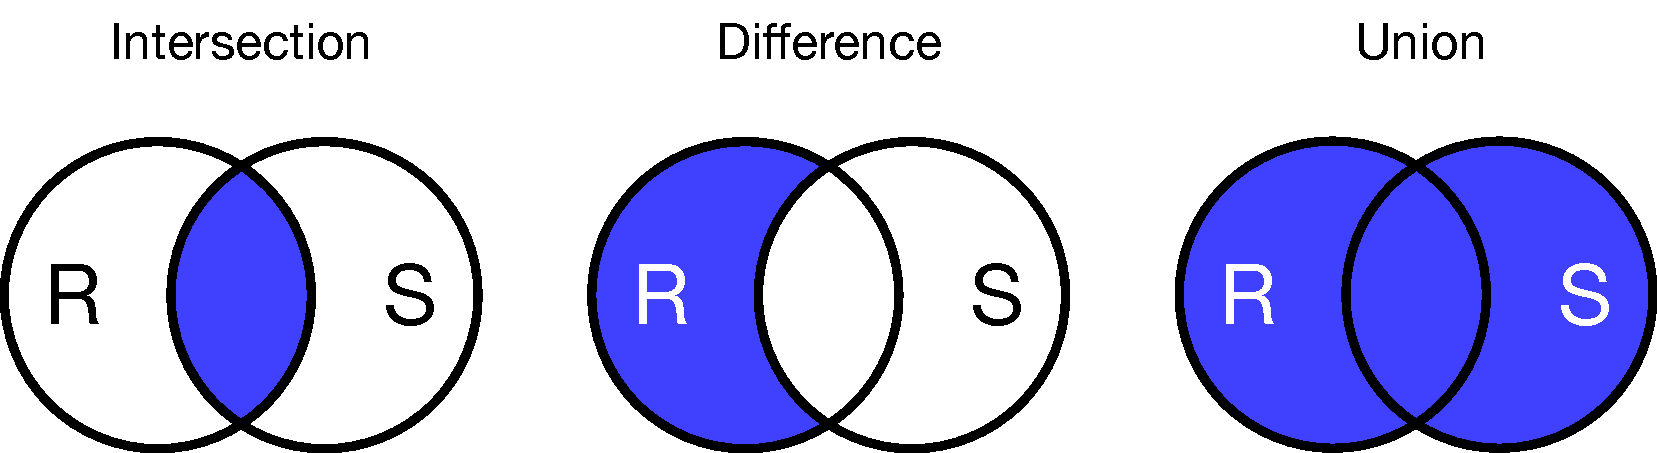
\includegraphics[width=1\textwidth]{./lectRCRA/setOps.pdf}}
\begin{itemize}
\item[?] What is the maximum number of tuples in $R \cup S$?
\begin{enumerate}[A]
\item |R|
\item  |S|
\item |R| $\times$ |S|
\item |R| + |S| % this one
\end{enumerate}
\end{itemize}

\end{frame}

%***********************************************************

\begin{frame}{Union Example}

FACULTY (\underline{NETID}, LASTNAME, FIRSTNAME, HIREDATE, TERMDATE)

STUDENT (\underline{NETID}, LASTNAME, FIRSTNAME)

\begin{noindentitemize}
\item[?] What are the names of all the people at Rice?
\end{noindentitemize}
\end{frame}
%***********************************************************

\begin{frame}{Union Example}

FACULTY (\underline{NETID}, LASTNAME, FIRSTNAME, HIREDATE, TERMDATE)

STUDENT (\underline{NETID}, LASTNAME, FIRSTNAME)

\begin{noindentitemize}
\item What are the names of all the people at Rice?
\item $\pi_{lastname, firstname}(\STUDENT) \cup\ \pi_{lastname, firstname}(\FACULTY)$
\end{noindentitemize}
\end{frame}
%***********************************************************

\begin{frame}{Union Example}

FACULTY (\underline{NETID}, LASTNAME, FIRSTNAME, HIREDATE, TERMDATE)

STUDENT (\underline{NETID}, LASTNAME, FIRSTNAME)

\begin{noindentitemize}
\item What are the names of all the people at Rice?
\item $\pi_{lastname, firstname}(\STUDENT) \cup\ \pi_{lastname, firstname}(\FACULTY)$
\item[?] Why do we project out lastname, firstname?
% because attributes have to match in type and quantity to do a set op
\end{noindentitemize}
\end{frame}

%***********************************************************
%
%\begin{frame}{Union Visualization}. 
%
%FACULTY\\
%\begin{tabular}{|p{2cm}|p{2cm}|p{2cm}|p{2cm}|p{2cm}|}  \hline
%  \cellcolor{black}\underline{NETID} & LASTNAME & FIRSTNAME &   \cellcolor{black}HIREDATE &  \cellcolor{black}TERMDATE\\ \hline
%   \cellcolor{black} & Myers & Risa &   \cellcolor{black}&   \cellcolor{black}\\ \hline
%    \cellcolor{black}& Jermaine & Chris &   \cellcolor{black}&  \cellcolor{black} \\ \hline
%    \cellcolor{black}& Greiner & John &   \cellcolor{black}&  \cellcolor{black} \\ \hline
%    \cellcolor{black}& Cooper & Keith &   \cellcolor{black}&  \cellcolor{black} \\ \hline
%    \cellcolor{black}& Nakhleh & Luay &   \cellcolor{black}&  \cellcolor{black} \\ \hline
% \end{tabular}
%
%STUDENT \\
%\begin{tabular}{|p{2cm}|p{2cm}|p{2cm}|}  \hline
%  \cellcolor{black}\underline{NETID}&LASTNAME & FIRSTNAME \\ \hline
%    \cellcolor{black} & Jones & Robert  \\ \hline
% \end{tabular}
%
%
%
%\end{frame}


%***********************************************************

\begin{frame}{Intersection Example}

FACULTY (\underline{NETID}, LASTNAME, FIRSTNAME, HIREDATE, TERMDATE)

STUDENT (\underline{NETID}, LASTNAME, FIRSTNAME)

\begin{noindentitemize}
\item[?] Who has been both a student and a faculty member?
\end{noindentitemize}
\end{frame}
%***********************************************************

\begin{frame}{Intersection Example}

FACULTY (\underline{NETID}, LASTNAME, FIRSTNAME, HIREDATE, TERMDATE)

STUDENT (\underline{NETID}, LASTNAME, FIRSTNAME)

\begin{noindentitemize}
\item Who has been both a student and a faculty member?
\item $\pi_{lastname, firstname}(\STUDENT) \cap\ \pi_{lastname, firstname}(\FACULTY)$
\end{noindentitemize}
\end{frame}

%***********************************************************
\begin{frame}{Difference Example}

FACULTY (\underline{NETID}, LASTNAME, FIRSTNAME, HIREDATE, TERMDATE)

STUDENT (\underline{NETID}, LASTNAME, FIRSTNAME)

\begin{noindentitemize}
\item $\pi_{lastname, firstname}(\FACULTY) -\ \pi_{lastname, firstname}(\STUDENT)$
\item[?] What does this expression represent (in English)?
\end{noindentitemize}
\end{frame}

%***********************************************************
\begin{frame}{Difference Example}

FACULTY (\underline{NETID}, LASTNAME, FIRSTNAME, HIREDATE, TERMDATE)

STUDENT (\underline{NETID}, LASTNAME, FIRSTNAME)

\begin{noindentitemize}
\item $\pi_{lastname, firstname}(\FACULTY) -\ \pi_{lastname, firstname}(\STUDENT)$
\item Faculty who have never been students
\end{noindentitemize}
\end{frame}



%***********************************************************

\begin{frame}{Set-Based Operations}

LIKES (DRINKER, COFFEE)

FREQUENTS (DRINKER, CAFE)

SERVES (CAFE, COFFEE)

\begin{noindentitemize}
\item[?] Who does not like `Cold Brew' coffee?
\end{noindentitemize}
\end{frame}

%***********************************************************


\begin{frame}{Set-Based Operations}

LIKES (DRINKER, COFFEE)

FREQUENTS (DRINKER, CAFE)

SERVES (CAFE, COFFEE)

\begin{noindentitemize}
\item Who does not like `Cold Brew' coffee?
	\begin{noindentitemize2}
	\item $\CBGOOD \leftarrow \pi_{\DRINKER} (\sigma_{\COFFEE = \CB}(\LIKES))$
	\item $(\pi_{\DRINKER} (\FREQUENTS)) - \CBGOOD$
	\end{noindentitemize2}
\item[?] Why use \FREQUENTS\ instead of \LIKES?
% because some people might go to a Cafe just to hang out
% better is to use union of drinkers and frequents and likes
\end{noindentitemize}
\end{frame}
%***********************************************************
\begin{frame}{More Set-Based Examples}

LIKES (DRINKER, COFFEE)

FREQUENTS (DRINKER, CAFE)

SERVES (CAFE, COFFEE)
\begin{enumerate}
\item Which cafes serve Cold Brew? 
\item Who goes to cafes serving Cold Brew?
\item Who goes to a cafe that both Risa and Chris go to?
\item Who avoids Risa at all costs?
\end{enumerate}
\end{frame}


%***********************************************************
\begin{frame}{More Set-Based Examples}

LIKES (DRINKER, COFFEE)

FREQUENTS (DRINKER, CAFE)

SERVES (CAFE, COFFEE)
\begin{enumerate}
\item Which cafes serve Cold Brew?
\item[] $\pi_{CAFE}(\sigma_{COFFEE = \textquotesingle{Cold\ Brew}\textquotesingle}(\SERVES))$
\end{enumerate}
\end{frame}

%***********************************************************
\begin{frame}{More Set-Based Examples}

LIKES (DRINKER, COFFEE)

FREQUENTS (DRINKER, CAFE)

SERVES (CAFE, COFFEE)
\begin{enumerate}
\setcounter{enumi}{1}
\item Who goes to cafes serving Cold Brew?
\item[] $\pi_{DRINKER}(\sigma_{COFFEE = \textquotesingle{Cold\ Brew}\textquotesingle}(\SERVES * \FREQUENTS))$
\end{enumerate}
\end{frame}

%***********************************************************
\begin{frame}{More Set-Based Examples}

LIKES (DRINKER, COFFEE)

FREQUENTS (DRINKER, CAFE)

SERVES (CAFE, COFFEE)
\begin{enumerate}
\setcounter{enumi}{2}
\item Who goes to a cafe that both Risa and Chris go to?
\item[] $C \leftarrow \pi_{CAFE}(\sigma_{DRINKER=\textquotesingle{Risa}\textquotesingle}(\FREQUENTS))\ $\\
\hspace{2em}$\cap\ \pi_{CAFE}(\sigma_{DRINKER=\textquotesingle{Chris}\textquotesingle}(\FREQUENTS))$\\
$\pi_{DRINKER}(\FREQUENTS * C)$
\end{enumerate}
\end{frame}

%***********************************************************
\begin{frame}{More Set-Based Examples}

LIKES (DRINKER, COFFEE)

FREQUENTS (DRINKER, CAFE)

SERVES (CAFE, COFFEE)
\begin{enumerate}
\setcounter{enumi}{3}
\item Who avoids Risa at all costs?
\item[] Want: Cafes each person goes to - cafes Risa goes to
\item[] $RCAFES \leftarrow  \pi_{CAFE}(\sigma_{DRINKER=\textquotesingle{Risa}\textquotesingle}(\FREQUENTS))$\\
\item[] $\pi_{DRINKER}(\FREQUENTS) - \pi_{DRINKER}(\FREQUENTS * RCAFES)$
\end{enumerate}
\end{frame}



%***********************************************************
%
%\begin{frame}{Complicated Set-Based Example}
%
%LIKES (DRINKER, COFFEE)
%
%FREQUENTS (DRINKER, CAFE)
%
%SERVES (CAFE, COFFEE)
%
%\begin{noindentitemize}
%\item[?] Who only goes to cafes where they can get a coffee they like?
%\end{noindentitemize}
%\end{frame}

%***********************************************************

\begin{frame}{Complicated Set-Based Example}

LIKES (DRINKER, COFFEE)

FREQUENTS (DRINKER, CAFE)

SERVES (CAFE, COFFEE)

\begin{noindentitemize}
\item Who only goes to cafes where they can get a coffee they like?
	\begin{noindentitemize2}
	\item Use `all people' $-$ `those who go to a cafe where they can't get a coffee they like'
	\item $\ALLPEEPS \leftarrow \pi_{\DRINKER}(\FREQUENTS)$
	\item How about `those who go to a cafe where they can't get a coffee they like'?
	\item Use FREQUENTS $-$ `DRINKER, CAFE combos where the person can get a coffee they like'
	\item $\GOODCOFFEE \leftarrow \pi_{\DRINKER, \CAFE}(\LIKES * \SERVES)$
	\end{noindentitemize2}
\item Then the answer is 
	\begin{noindentitemize2}
	\item $\ALLPEEPS - \pi_{\DRINKER}(\FREQUENTS - \GOODCOFFEE)$
	\end{noindentitemize2}
\end{noindentitemize}
\end{frame}
%***********************************************************

\begin{frame}{Review}
\begin{enumerate}
\item If R has 3 tuples and S has 2 tuples, R $\times$ S returns how many tuples?
\begin{enumerate}[A]
\item 2
\item 3
\item 6
\item None of the above
\end{enumerate}
\end{enumerate}
True / False
\begin{enumerate}
\setcounter{enumi}{1}
\item The most commonly used type of join is Cartesian product
\item Attribute names must match to join relations on them
\item When you perform a join, the join column is always duplicated
\item Each relation may be used at most 1 time per query
\item Union and Intersection can operate on relations with different numbers or types of attributes

\end{enumerate}
\end{frame}
%1. 6
%2. F
%3. F
%4. Sometimes : not in natural joins
%5. but have to rename
%6. F

%***********************************************************

\begin{frame}{Wrap up}
\begin{enumerate}
\item What is Relational Algebra?
%abstract machine of relational dbs
\item Why does it matter?
% gets us thinking like SQL
\end{enumerate}

\begin{itemize}
	\item[?] How can we use what we learned today?
	\vspace{2em}
	\item[?] What do we know now that we didn't know before?
\end{itemize}


\end{frame}


\end{document}
